\documentclass[a4paper,twoside,12pt,fleqn]{article}
\usepackage [reqno] {amsmath}
\usepackage{amsfonts,amstext}
\usepackage{amsmath}
\usepackage{amsthm}
\usepackage{german}
\usepackage{graphicx}
\usepackage{fullpage}
\usepackage{pgf}
\usepackage{tikz}
\usetikzlibrary{arrows, automata}

\newcommand{\ABGABEDATUM}{am 11. Mai 2018 bis 10 Uhr}

\newcounter{AUFGNR}
\setcounter{AUFGNR}{1}
\newcommand{\AUFGABE}[2]{\vspace{0.3cm}\item[Aufgabe~\arabic{AUFGNR}]\stepcounter{AUFGNR} #1\hfill\emph{#2}}


\newcommand{\floor}[1]{\left\lfloor{#1}\right\rfloor}
\newcommand{\ceil}[1]{\left\lceil{#1}\right\rceil}
\newcommand{\half}[1]{\frac{#1}{2}}

\newcommand{\N}{\mathbb{N}}
\newtheorem*{antwort}{Antwort}


\renewcommand{\labelenumi}{(\alph{enumi})}
\renewcommand{\labelenumii}{(\roman{enumii})}


\begin{document}
\pagestyle{empty}

\noindent
\large
\textbf{Grundlagen der theoretischen Informatik}\hfill SoSe 2018 \\[0.5ex]
\normalsize
Anton Oehler, Jona Rex

\medskip\hrule

\smallskip
\noindent
\textbf{Abgabe} \ABGABEDATUM



\begin{description}
	% AUFGABE 1
	\AUFGABE{Deterministische endliche Automaten}{10 Punkte}
	% 1 a
	\begin{figure}[htbp]
		\centering
		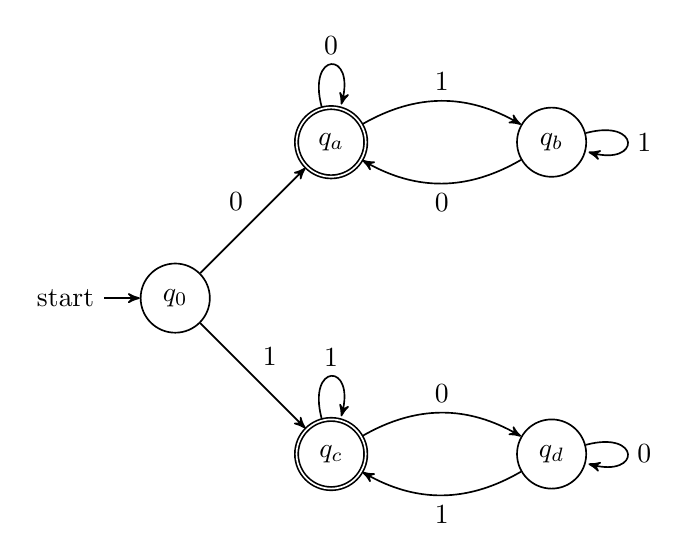
\begin{tikzpicture}[->,>=stealth',auto,node distance=2.8cm,semithick]
			\node[state, initial]                     (S) {$q_0$};
			\node[state, above right of=S, accepting] (A) {$q_a$};
			\node[state, right of=A]                  (B) {$q_b$};
			\node[state, below right of=S, accepting] (C) {$q_c$};
			\node[state, right of=C]                  (D) {$q_d$};
			\draw (S) edge             node {0} (A);
			\draw (A) edge[loop above] node {0} (A);
			\draw (A) edge[bend left]  node {1} (B);
			\draw (B) edge[loop right] node {1} (B);
			\draw (B) edge[bend left]  node {0} (A);
			\draw (S) edge             node {1} (C);
			\draw (C) edge[loop above] node {1} (C);
			\draw (C) edge[bend left]  node {0} (D);
			\draw (D) edge[loop right] node {0} (D);
			\draw (D) edge[bend left]  node {1} (C);
		\end{tikzpicture}
		\caption{Teilaufgabe a)}
	\end{figure}
	% 1 b
	\begin{figure}[htbp]
		\centering
		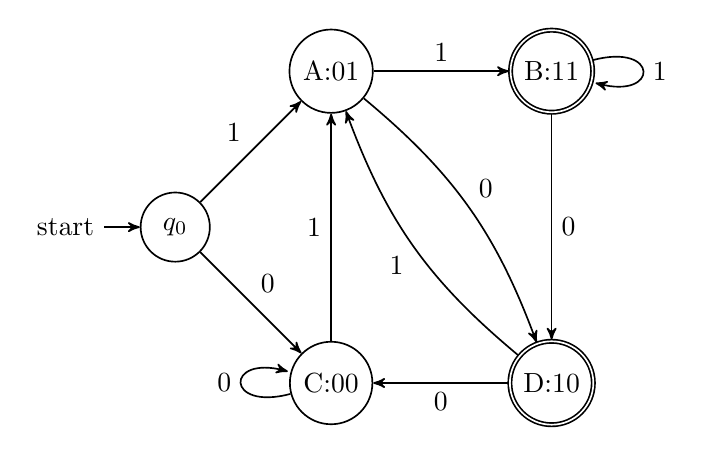
\begin{tikzpicture}[->,>=stealth',auto,node distance=2.8cm,semithick]
			\node[state, initial]                     (S) {$q_0$};
			\node[state, above right of=S]      (A) {A:$01$};
			\node[state, right of=A, accepting] (B) {B:$11$};
			\node[state, below right of=S]      (C) {C:$00$};
			\node[state, right of=C, accepting] (D) {D:$10$};
			\draw (S) edge               node {1} (A);
			\draw (S) edge               node {0} (C);
			\draw (A) edge               node {1} (B);
			\draw (A) edge[bend left=15] node {0} (D);
			\draw (B) edge[loop right]   node {1} (B);
			\draw (B) edge               node {0} (D);
			\draw (C) edge               node {1} (A);
			\draw (C) edge[loop left]    node {0} (C);
			\draw (D) edge[bend left=15] node {1} (A);
			\draw (D) edge               node {0} (C);
		\end{tikzpicture}
		\caption{Teilaufgabe b)}
	\end{figure}
	% a c
	\begin{figure}[htbp]
		\centering
		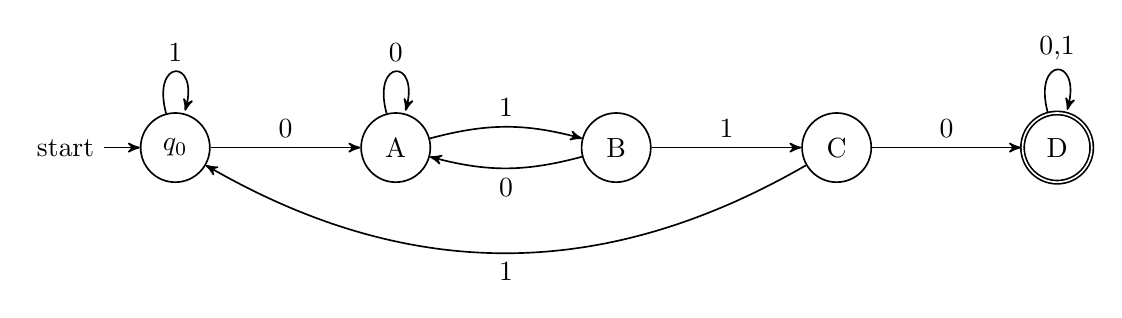
\begin{tikzpicture}[->,>=stealth',auto,node distance=2.8cm,semithick]
			\node[state, initial]    (S) {$q_0$};
			\node[state, right of=S] (A) {A};
			\node[state, right of=A] (B) {B};
			\node[state, right of=B] (C) {C};
			\node[state, right of=C, accepting] (D) {D};
			\draw (S) edge               node {0} (A);
			\draw (S) edge[loop above]   node {1} (S);
			\draw (A) edge[loop above]   node {0} (A);
			\draw (A) edge[bend left=15] node {1} (B);
			\draw (B) edge[bend left=15] node {0} (A);
			\draw (B) edge               node {1} (C);
			\draw (C) edge               node {0} (D);
			\draw (C) edge[bend left]    node {1} (S);
			\draw (D) edge[loop above]   node {0,1} (D);
		\end{tikzpicture}
		\caption{Teilaufgabe c)}
	\end{figure}
	% a d
	\begin{figure}[htbp]
		\centering
		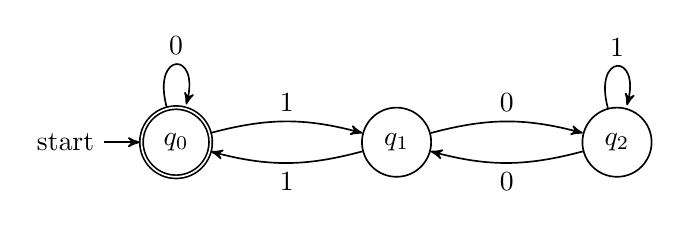
\begin{tikzpicture}[->,>=stealth',auto,node distance=2.8cm,semithick]
			\node[state, initial, accepting] (0) {$q_0$};
			\node[state, right of=0]         (1) {$q_1$};
			\node[state, right of=1]         (2) {$q_2$};
			\draw (0) edge[loop above]   node {0} (0);
			\draw (0) edge[bend left=15] node {1} (1);
			\draw (1) edge[bend left=15] node {0} (2);
			\draw (1) edge[bend left=15] node {1} (0);
			\draw (2) edge[bend left=15] node {0} (1);
			\draw (2) edge[loop above]   node {1} (2);
		\end{tikzpicture}
		\caption{Teilaufgabe d)}
	\end{figure}
	% AUFGABE 2
	\AUFGABE{Potenzmengenkonstruktion}{10 Punkte}
	\begin{figure}[htbp]
		\centering
		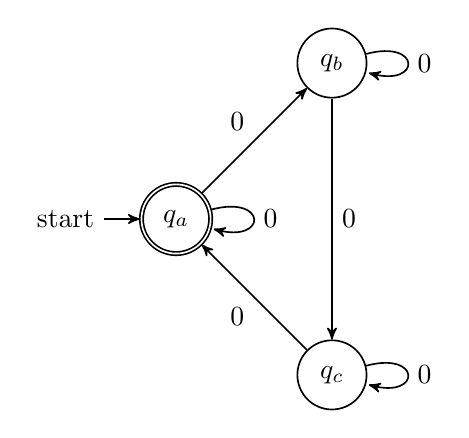
\begin{tikzpicture}[->,>=stealth',auto,node distance=2.8cm,semithick]
			\node[state, initial, accepting] (a) {$q_a$};
			\node[state, above right of=a]   (b) {$q_b$};
			\node[state, below right of=a]   (c) {$q_c$};
			\draw (a) edge[loop right] node {0} (a);
			\draw (a) edge             node {0} (b);
			\draw (b) edge[loop right] node {0} (b);
			\draw (b) edge             node {0} (c);
			\draw (c) edge[loop right] node {0} (c);
			\draw (c) edge             node {0} (a);
		\end{tikzpicture}
		\caption{Zustandsdiagramm von $M$ (NEA)}
	\end{figure}
	\begin{figure}[htbp]
		\centering
		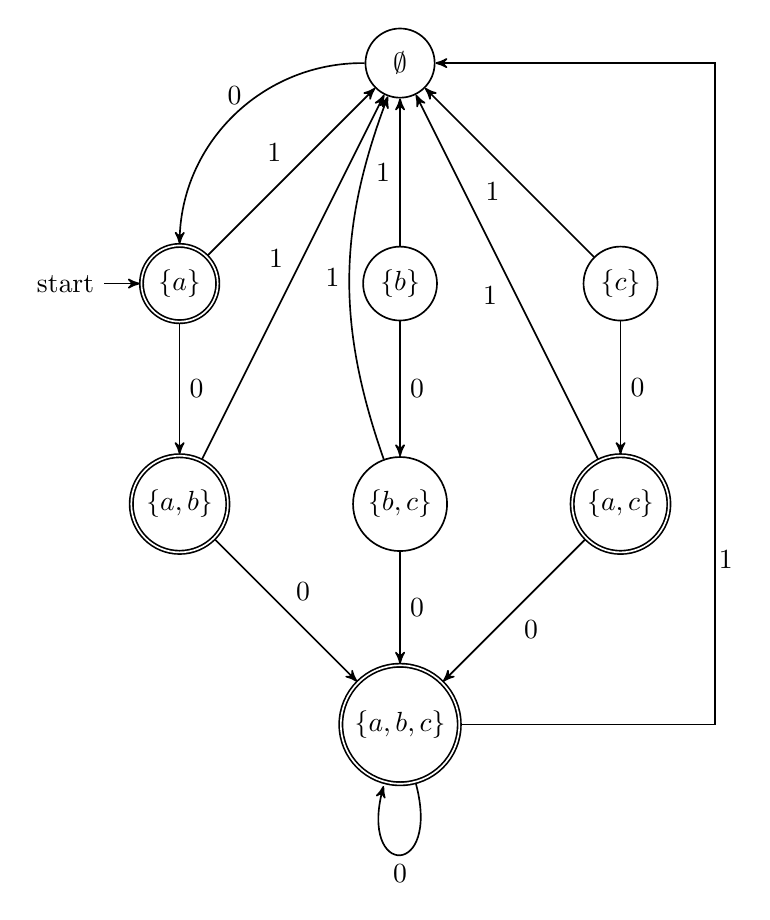
\begin{tikzpicture}[->,>=stealth',auto,node distance=2.8cm,semithick]
			\node[state, accepting, initial    ] (a) {$\{a\}$};
			\node[state,            right of=a ] (b) {$\{b\}$};
			\node[state,            right of=b ] (c) {$\{c\}$};
			\node[state, accepting, below of=a ] (ab) {$\{a,b\}$};
			\node[state,            below of=b ] (bc) {$\{b,c\}$};
			\node[state, accepting, below of=c ] (ac) {$\{a,c\}$};
			\node[state, accepting, below of=bc] (abc) {$\{a,b,c\}$};
			\node[state,            above of=b ] (e) {$\emptyset$};
			\draw (a)   edge             node {0} (ab);
			\draw (b)   edge             node {0} (bc);
			\draw (c)   edge             node {0} (ac);
			\draw (ab)  edge             node {0} (abc);
			\draw (bc)  edge             node {0} (abc);
			\draw (ac)  edge             node {0} (abc);
			\draw (abc) edge[loop below] node {0} (abc);
			\draw (e)   edge[bend right=45,above] node {0} (a);
			\draw (a)   edge               node {1} (e);
			\draw (b)   edge               node {1} (e);
			\draw (c)   edge               node {1} (e);
			\draw (ab)  edge               node {1} (e);
			\draw (bc)  edge[bend left=20] node {1} (e);
			\draw (ac)  edge               node {1} (e);
			\draw (abc) -- ++(4,0) |- node[very near start,xshift=1em] {1} (e);
		\end{tikzpicture}
		\caption{Zustandsdiagramm von $M$ (DEA, vollst"andig)}
	\end{figure}
	\begin{figure}[htbp]
		\centering
		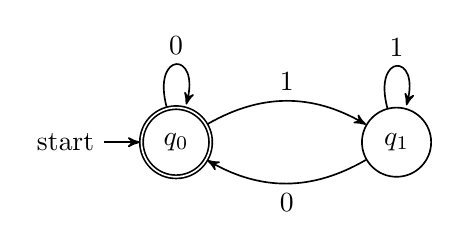
\begin{tikzpicture}[->,>=stealth',auto,node distance=2.8cm,semithick]
			\node[state, accepting, initial] (a) {$q_0$};
			\node[state, right of=a]         (b) {$q_1$};
			\draw (a) edge[loop above] node {0} ();
			\draw (a) edge[bend left]  node {1} (b);
			\draw (b) edge[bend left]  node {0} (a);
			\draw (b) edge[loop above] node {1} ();
		\end{tikzpicture}
		\caption{Zustandsdiagramm von $M$ (DEA, vereinfacht)}
	\end{figure}

	% AUFGABE 3
	\AUFGABE{NEAs mit mehreren Startzust"anden}{10 Punkte}
	\begin{enumerate}
		\item NEAs mit mehreren Startzust"anden sind wie NEAs mit einem
		Startzustand, nur wird statt einem Startzustand $q_0$ eine
		Menge von Startzust"anden $Q_0$ verwendet. Jeder NEA mit
		einem Startzustand wird dann mit $Q_0 = \{q_0\}$ dargestellt.
		\item Jeder NEA mit mehreren Startzust"anden l"asst sich als
		NEA mit einem Startzustand darstellen, indem analog zur
		Konstruktion von DEAs aus NEAs die Potenzmengenkonstruktion
		verwendet wird. Zu jeder Untermenge der Menge aller Zust"ande
		wird ein Zustand angelegt, die "Uberg"ange werden analog zur
		Potenzmengenkonstruktion von NEA zu DEA gew"ahlt.
		Nun gibt es einen Zustand $\{q_0, q_1, q_2, \dots\}, q_i \in Q_0$,
		der alle Startzust"ande des Urspungs-NEA enth"alt. Dieser wird
		zum Startzustand des ``Potenzmengen-NEAs``. Der Beweis, dass
		die Potenzmengenkonstruktion die selbe Sprache repr"asentiert,
		ist von der Potenzmengenkonstruktion von NEA zu DEA zu entnehmen.
	\end{enumerate}
\end{description}
\end{document}
